\documentclass[greek]{beamer}
%\usepackage{fontspec}
\usepackage{amsmath,amsthm}
\usepackage{unicode-math}
\usepackage{xltxtra}
\usepackage{graphicx}
\usetheme{CambridgeUS}
\usecolortheme{seagull}
\usepackage{hyperref}
\usepackage{ulem}
\usepackage{xgreek}
\usepackage{pgfpages}
\usepackage{tikz}
%\setbeameroption{show notes on second screen}
%\setbeameroption{show only notes}

\setsansfont{Noto Serif}

\usepackage{multicol}

\usepackage{appendixnumberbeamer}

\setbeamercovered{transparent}
\beamertemplatenavigationsymbolsempty

\title{Συναρτήσεις}
\subtitle{Θεώρημα Bolzano}
\author[Λόλας]{Κωνσταντίνος Λόλας}
\date{}

\begin{document}

\begin{frame}
 \titlepage
\end{frame}

\section{Θεωρία}
\begin{frame}{Challenge}
 \begin{itemize}
  \item<1-> Φτιάξτε άξονες
  \item<2-> Σημειώστε ένα σημείο $Α$ με θετική τεταγμένη και ένα σημείο $Β$ με αρνητική
  \item<3-> Σχηματίστε συνάρτηση στο $[α,β]$ χωρίς να περάσετε από τον άξονα $x'x$
 \end{itemize}
 \onslide<4-> Συμπέρασμα...
\end{frame}

\begin{frame}{Χωρίς πολλά πολλά...}
 \begin{block}{Θεώρημα Bolzano}
  Έστω μια συνάρτηση $f$ ορισμένη σε κλειστό διάστημα $[α,β]$. Αν:
  \begin{itemize}
   \item η $f$ είναι συνεχής στο $[α,β]$ και
   \item $f(α)\cdot f(β)<0$,
  \end{itemize}
  τότε υπάρχει $x_0\in (α,β)$ τέτοιο ώστε $f(x_0)=0$
 \end{block}
\end{frame}

\begin{frame}{Παρατηρήσεις}
 \begin{itemize}
  \item<1-> ΔΕΝ είναι τρόπος επίλυσης εξισώσεων
  \item<2-> ΔΕΝ βρίσκει - εντοπίζει ρίζες
  \item<3-> ΔΕΝ τις μετράει σε πλήθος
 \end{itemize}
 \onslide<4->Το μόνο που κάνει είναι να σε πληροφορεί ότι ΣΙΓΟΥΡΑ έχει ρίζα μια συνάρτηση. \onslide<5-> ΜΟΝΟ
\end{frame}

\begin{frame}{Τεστ μνήμης - ικανοτήτων}
 Πώς επιλύουμε εξισώσεις αλγεβρικά?
 \begin{itemize}
  \item<1-> Προφανής ρίζα
  \item<2-> Λύνουμε ως προς $x$
  \item<3-> Παραγοντοποίηση
  \item<4-> 1-1
 \end{itemize}
\end{frame}

\section{Ασκήσεις}
\subsection{Άσκηση 1}
\begin{frame}[label=Άσκηση1]{Εξάσκηση 1}
 Να αποδείξετε ότι:
 \begin{enumerate}
  \item<1-> Η συνάρτηση $f(x)=x^3+x-1$ ικανοποιεί τις υποθέσεις του θεωρήματος Bolzano στο διάστημα $[0,1]$.
  \item<2-> Η εξίσωση $x^3+x-1=0$ έχει μία τουλάχιστον ρίζα στο διάστημα $(0,1)$.
 \end{enumerate}

 %\hyperlink{Λύση1}{\beamerbutton{Λύση}}
\end{frame}

\subsection{Άσκηση 2}
\begin{frame}[label=Άσκηση2]{Εξάσκηση 2}
 Να αποδείξετε ότι υπάρχει ένα τουλάχιστον $x_0\in (0,1)$ τέτοιο ώστε $x_0^2+3x_0=e^{x_0}+1$.

 %\hyperlink{Λύση2}{\beamerbutton{Λύση}}
\end{frame}

\subsection{Άσκηση 3}
\begin{frame}[label=Άσκηση3]{Εξάσκηση 3}
 Έστω $f:\mathbb{R}\to\mathbb{R}$ μία συνάρτηση η οποία είναι συνεχής με $f(\mathbb{R})=(0,1)$. Να αποδείξετε ότι η εξίσωση $f(x)=x-1$ έχει μία τουλάχιστον ρίζα στο διάστημα $(1,2)$.

 %\hyperlink{Λύση3}{\beamerbutton{Λύση}}
\end{frame}

\subsection{Άσκηση 4}
\begin{frame}[label=Άσκηση4]{Εξάσκηση 4}
 Να αποδείξετε ότι η εξίσωση $\frac{e^x}{x-2}+\frac{x^2+1}{x-1}=0$ έχει μία τουλάχιστον ρίζα στο διάστημα $(1,2)$.

 %\hyperlink{Λύση4}{\beamerbutton{Λύση}}
\end{frame}

\subsection{Άσκηση 5}
\begin{frame}[label=Άσκηση5]{Εξάσκηση 5}
 Να αποδείξετε ότι υπάρχει μοναδικό $x_0\in (0,1)$ τέτοιο ώστε $e^{x_0}+x_0=2$

 %\hyperlink{Λύση5}{\beamerbutton{Λύση}}
\end{frame}

\subsection{Άσκηση 6}
\begin{frame}[label=Άσκηση6]{Εξάσκηση 6}

 Δίνονται οι συναρτήσεις $f(x)=\ln x$ και $g(x)=\frac{1}{x}$. Να αποδείξετε ότι οι $C_f$ και $C_g$ στο διάστημα $(1,e)$ έχουν ένα ακριβώς κοινό σημείο.

 %\hyperlink{Λύση6}{\beamerbutton{Λύση}}
\end{frame}

\subsection{Άσκηση 7}
\begin{frame}[label=Άσκηση7]{Εξάσκηση 7}

 Να αποδείξετε ότι η εξίσωση $x^3-4x^2+2=0$ έχει δύο τουλάχιστον ρίζες στο διάστημα $(-1,1)$.

 %\hyperlink{Λύση7}{\beamerbutton{Λύση}}
\end{frame}

\subsection{Άσκηση 8}
\begin{frame}[label=Άσκηση8]{Εξάσκηση 8}
 Δίνεται το ορθογώνιο $ΟΑΒΓ$ του σχήματος και μία συνεχής συνάρτηση $f$ στο $[0,2]$ της οποίας η γραφική παράσταση βρίσκεται στο χωρίο που ορίζει το ορθογώνιο. Να αποδείξετε ότι η $C_f$ τέμνει τη διαγώνιο $ΑΓ$.


 \centering
 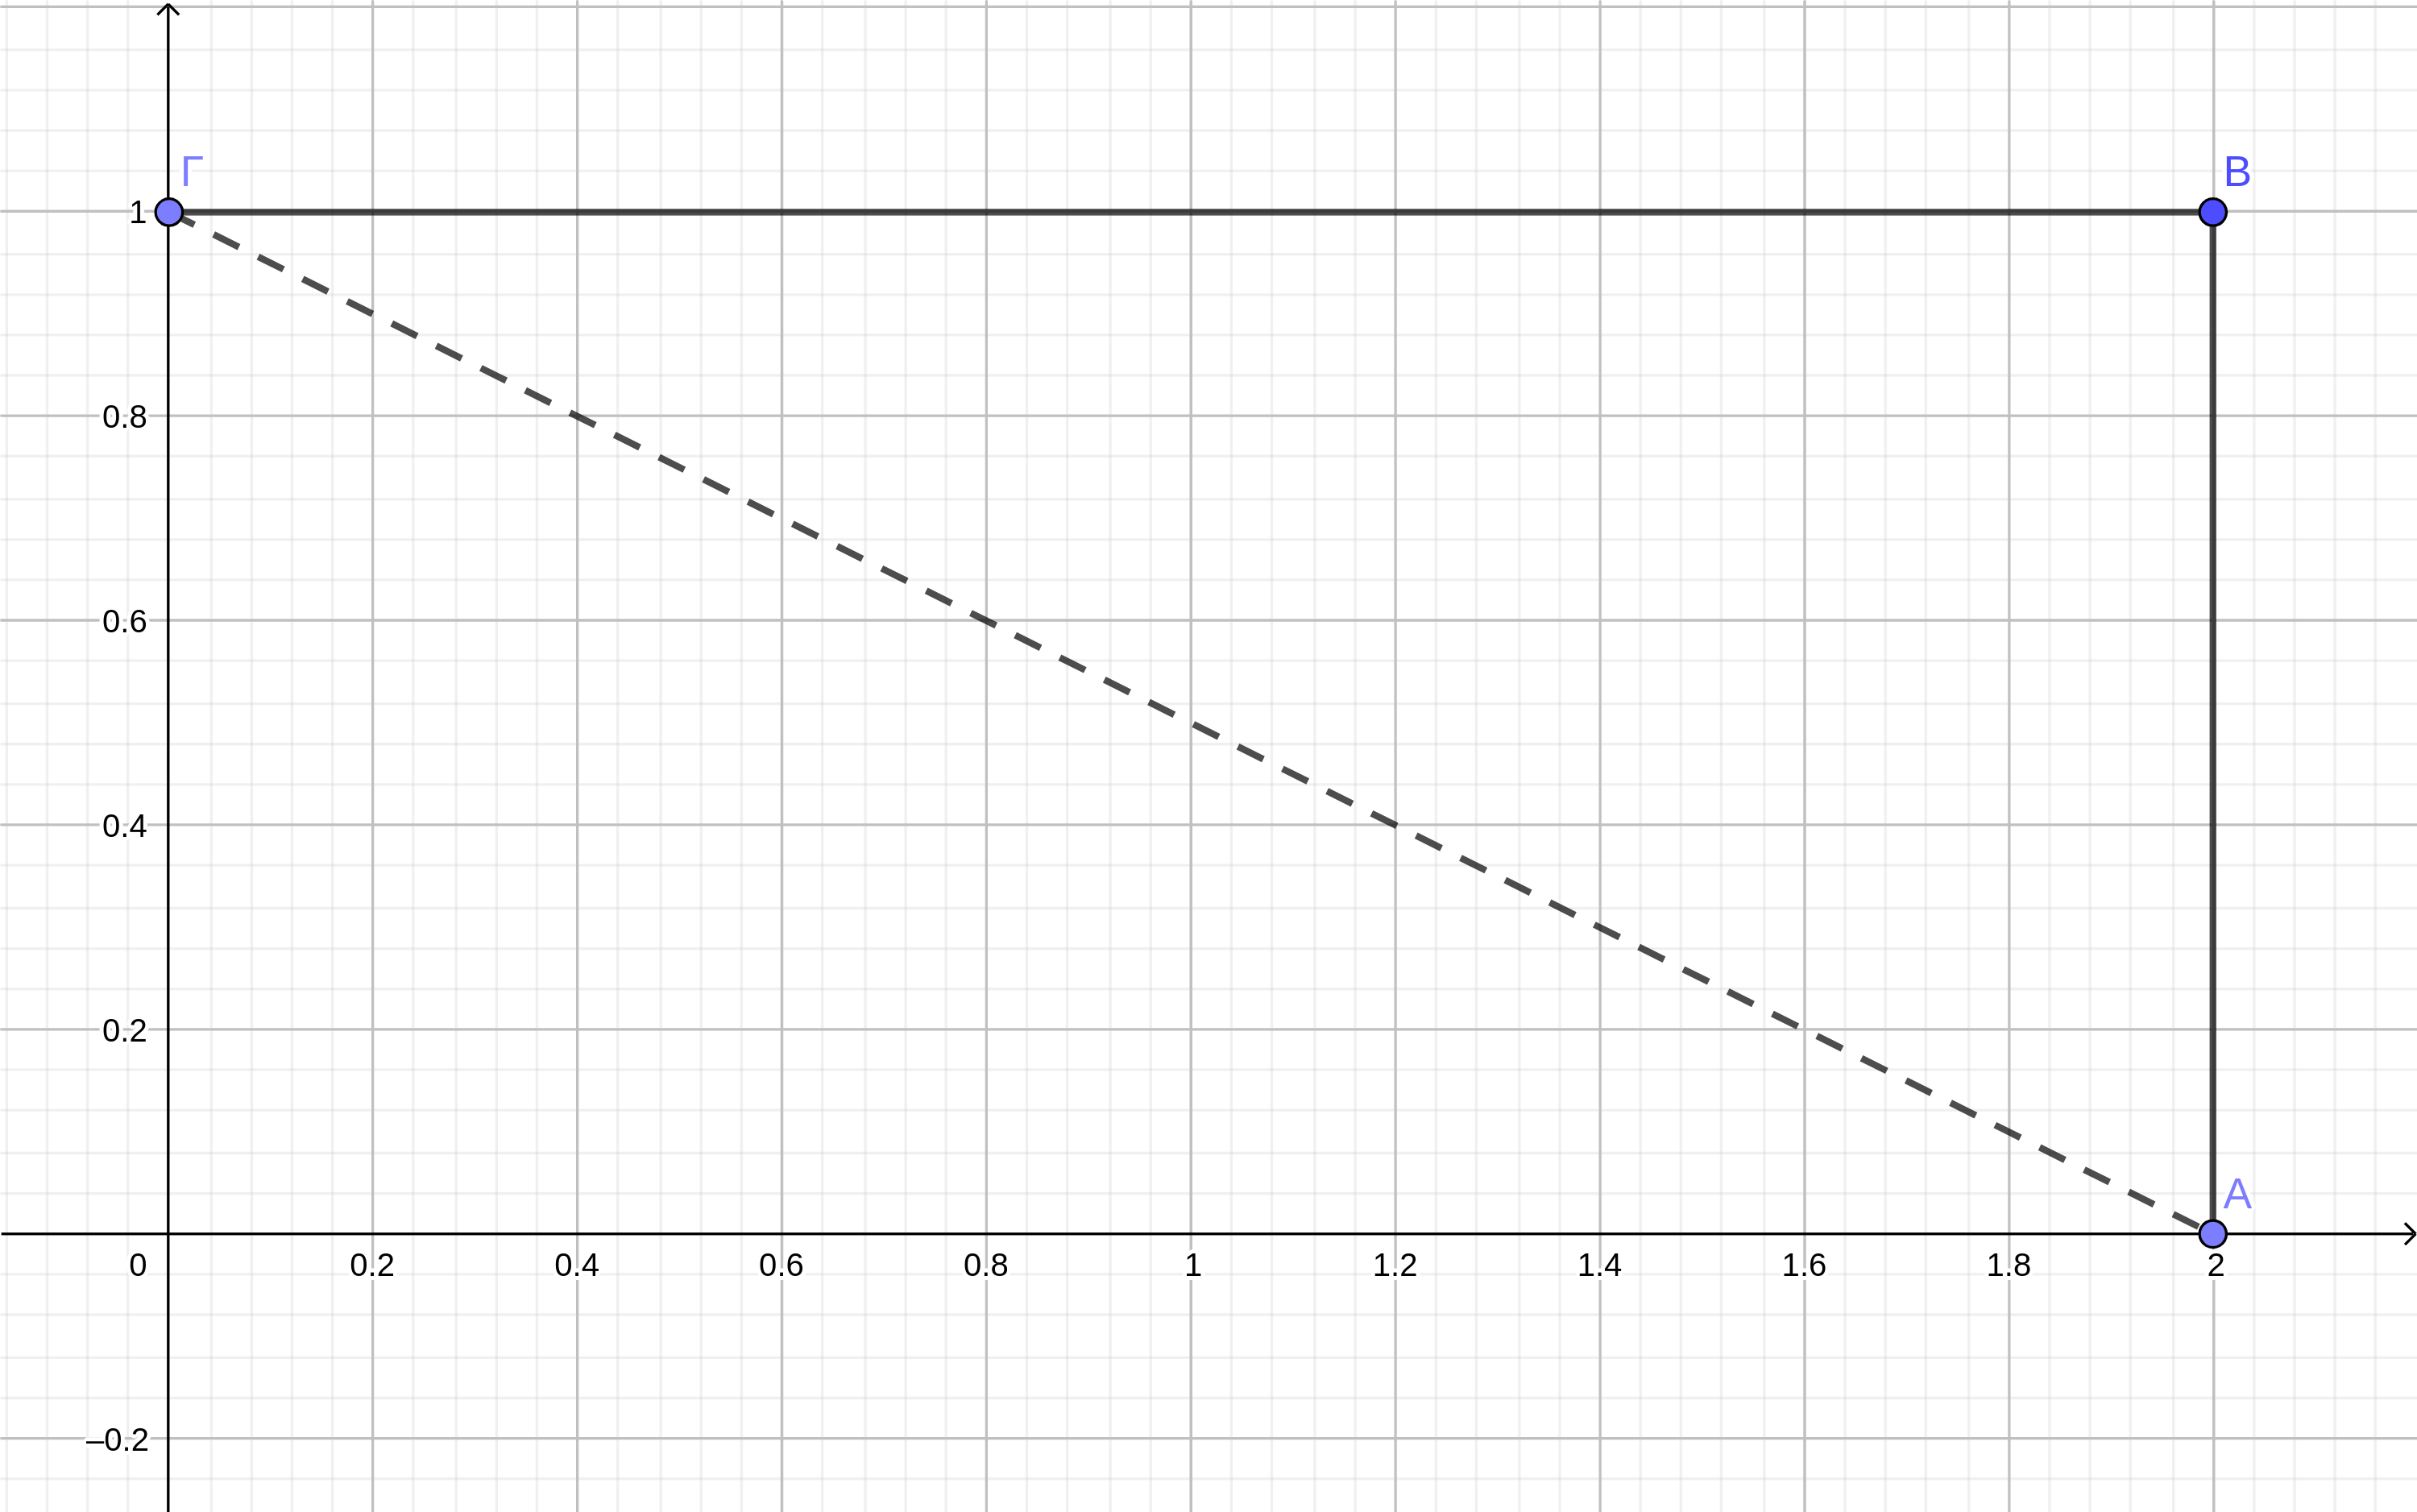
\includegraphics[width=0.5\textwidth]{"images/Bolzano.png"}

 %\hyperlink{Λύση8}{\beamerbutton{Λύση}}
\end{frame}

\subsection{Άσκηση 9}
\begin{frame}[label=Άσκηση9]{Εξάσκηση 9}
 Να δείξετε ότι η εξίσωση $\ln x=\frac{1}{x-1}$ έχει μία τουλάχιστον ρίζα στο διάστημα $(0,1)$.


 %\hyperlink{Λύση9}{\beamerbutton{Λύση}}
\end{frame}

\subsection{Άσκηση 10}
\begin{frame}[label=Άσκηση10]{Εξάσκηση 10}
 Έστω η συνεχής συνάρτηση $f:[0,1]\to\mathbb{R}$ με $-1<f(x)<0$, για κάθε $x\in [0,1]$. Να δείξετε ότι υπάρχει ένα τουλάχιστον $x_0\in (0,1)$ τέτοιο ώστε $f^2(x_0)=2f(x_0)+3x_0$

 %\hyperlink{Λύση10}{\beamerbutton{Λύση}}
\end{frame}

\section{}
\begin{frame}
 Στο moodle θα βρείτε τις ασκήσεις που πρέπει να κάνετε, όπως και αυτή τη παρουσίαση
\end{frame}

\end{document}
